\section{Active Pixel Sensor dosimeter}
\fig{aps}{esquematicos/aps.pdf}{APS dosimeter schematic}
The APS dosimeter has a structure similar to a pixel in a digital camera's image sensor.
It requires a low voltage supply when it's being irradiated,
which can be applied using a small battery.
Moreover, it can be quickly reset.
This enables its use for measurements with high temporal resolution.

This section starts by explaining the theory behind this dosimeter.
It then goes on to analyze how it was designed and optimized.
Finally, it presents measurements from the fabricated sensor,
and the conclusions that follow from these measurements.
%
\subsection{Principle of operation}
%
The APS functions by measuring the charge generated by radiation
striking a p-n junction's depletion region.
The junction's cathode is electrically isolated,
in order to accumulate the generated charge without leakage
(D1 in \figref{fig:aps}).
Before each measurement,
the circuit is reset by charging the cathode to
V$_{\text{DD}}$ with a brief turn-on of the reset transistor M1.
Radiation striking D1's depletion region interacts with the silicon lattice,
depositing energy through processes such as scattering and ionization (section~\ref{sec:radiacion}).
The resulting photons and secondary electrons create electron-hole pairs,
which drift in opposite directions due to the depletion region's built-in electric field.
Electrons accumulate in the cathode, gradually discharging it down to
\SI{0}{\volt}.
After irradiation,
the cathode voltage is measured through two stages of voltage followers M2 and M3.
These make up a circuit that replicates the input voltage at the output,
with a small offset.
Their purpose is to prevent the voltage measurement apparatus from
drawing charge from the cathode,
which would influence the measured value.
\subsection{Previous work}
Turchetta\cite{turchetta_monolithic_2001} describes an X ray APS dosimeter
fabricated using a standard \SI{0.6}{\micro\meter} CMOS process.
He builds a grid of pixels for use in particle tracking.
He exposes the sensor to X rays from \isotope{Fe}{55}
and \SI{15}{\giga\electronvolt} pions.
He writes the sensitivity in Volts per radiation-generated electron.
This number reaches up to \SI{15}{\micro\volt} per electron,
with an RMS noise equivalent to 15 electrons.
He presents an innovative layout which allows for almost all the wafer surface
to be sensitive to radiation.

Matis\cite{matis_charged_2003} also builds an APS array,
using a standard \SI{0.25}{\micro\meter} CMOS process.
He analyzes various signal processing schemes,
adding the output from multiple pixels
in order to collect all of the charge generated by an incoming particle.
He irradiates the sensor with X rays from
\isotope{Fe}{55},
and \SI{55}{\mega\electronvolt} protons.

Conti\cite{conti_use_2013} uses a commercial CMOS image sensor,
in order to study its response to X rays.
Specifically, he analyzes the 2D distribution generated by incoming photons,
along with other statistics.
His radiation source is a radiotherapy machine,
and he simulates the scattering caused by the patient
by using a block of acrylic as a phantom.
%
\subsection{Fabrication process}
Although fabrication of an integrated circuit comes after design,
all aspects of the design are conditioned by the characteristics of the fabrication process.
Specifically,
\begin{itemize}
    \item permissible voltage ranges,
    \item devices available in the Process Development Kit, and
    \item electrical characteristics of said devices
        (threshold voltages, parasitic capacitances, leakage currents, etc).
\end{itemize}

We designed and fabricated both the APS and FG dosimeters using X-FAB foundry's
XC06 process\cite{x-fab_0.6_2008}.
It is a \SI{0.6}{\micro\meter} technology node
(which roughly corresponds to the minimum CMOS gate length),
and is designed to operate with a \SI{5}{\volt} supply.
Its simplest variant provides one polysilicon layer and two metal layers.
It is possible to pay for additional process steps (which require more masks)
to add features such as low-doped regions for high voltage devices,
or etched windows for photosensitive devices.
\subsection{Reset}
The charge storage node is charged through the drain of a P-channel MOSFET,
whose source is connected to \vdd.
(\figref{fig:aps}).
During irradiation, its gate is driven to \vdd to turn it off.
In order to reset the dosimeter,
the gate is grounded.
This biases the PMOS in saturation,
charging the cathode at constant current and
linearly increasing $V_D$ up to $V_t$.
The PMOS then enters the triode region and starts conducting less current,
asymptotically charging the cathode to \vdd.
The use of a PMOS allows the cathode to reach \vdd,
while an NMOS could only reach $V_{dd}-V_{tn}$ before cutting off.

The reset PMOS is a minimum area transistor,
in order to contribute the minimum possible stray capacitance
to the cathode node.
This increases the sensitivity, as will be explained later.
\subsection{Response to incoming particles}
Each incoming particle deposits an average energy which is a function of
the particle's initial kinetic energy
\cite{berger_response_1969} (section~\ref{montecarloaps}).
A fraction $E$ of this energy goes to electron-hole pair production,
creating a charge
\begin{align*}
    Q &= \frac{qE}{E_i}
\end{align*}
with $q$ the electron charge and $E_i$ the pair production energy,
\SI{3.62}{\electronvolt} in silicon.
This charge shows up with a negative sign in the cathode, which lowers its voltage.
The change in voltage
\begin{align*}
    \Delta V &= \frac{\Delta Q}{C}
\end{align*}
is a function of the cathode node's total capacitance $C$.
This capacitance has contributions from
\begin{itemize}
    \item D1's junction,
    \item M1's drain-body junction,
    \item M2's gate, and
    \item metal lines near the node.
\end{itemize}
The total capacitance can be estimated by using the 
fabrication process specifications,
which include per-unit-area and per-unit-perimeter capacitances.
To this end, we used EDA (Electronic Design Automation) tools
which automatically estimate capacitances
based on the layout geometry
(section~\ref{section:diseno_aps}).
\subsection{Monte Carlo simulations}
\label{montecarloaps}
The APS dosimeter detects the energy that is deposited
in a narrow region of an integrated circuit.
For simulation purposes,
we simplified the die geometry down to three regions:
the SiO$_2$ surface, a Si substrate and
a Si sensitive region (\figref{fig:corteaps}).
\fig{corteaps}{figuras/aps/corte.pdf}
{Cross section of the geometry used to simulate the APS with Geant4 (not to scale).}
Dimensions were extracted from the APS layout and
from the process specifications.

Because Geant4 is mainly used for high-energy physics,
its default settings do not allow it to simulate secondary electrons with 
energies below \SI{250}{\electronvolt}.
In order to increase the accuracy at short length scales,
we used a list of interaction processes
which was put together for microelectronic simulations
\cite{Raine201497}.
It is capable of accurately simulating electrons down to energies of
\SI{16.7}{\electronvolt},
whose range in Si is on the order of \SI{0.1}{\nano\meter}.

The results can be seen in \figref{fig:energia1electron}.
% FIXME falta este gráfico usando
% ../tesis/figuras/aps/deposicion1electron001.pdf y demás
\fig{energia1electron}{figuras/aps/deposicion1electron_todos.pdf}
{Probability distribution for total energy deposited in the sensor (X axis),
simulated using Geant4.
Each plot corresponds to a difference kinetic energy for the incoming particle.
The mean deposited energy is in \figref{fig:energiadepositadaaps}.}
The increased response as incoming particle energy goes down
is due to the fact that slower electrons stop completely within the detector,
depositing all of their energy.
Electrons that are more energetic, however, only deposit a fraction of their total energy.
The mean deposited energy is in \figref{fig:energiadepositadaaps}.
\fig{energiadepositadaaps}{figuras/poster/aps_respuesta.pdf}
{Average response to an incoming electron
as a function of its initial energy.
It can be seen that lower-energy electrons stop completely inside the detector.
Crosses mark the results of Geant4 simulations,
while the solid line is the result of manual calculations using
data tabulated by NIST in ESTAR\cite{berger_estar_????}.}
For energies in the range of interest,
each incoming particle causes a shift of tens of mV.

The photon response is much smaller.
For the energy ranges of interest,
the resulting voltage change
is orders of magnitude below that of electrons with similar energies
(\figref{fig:aps_respuesta_foton}).
\fig{aps_respuesta_foton}{figuras/aps/respuesta_fotones.pdf}
{APS response to photons, calculated using values tabulated by NIST in XCOM\cite{suplee_xcom_2009}.}
\subsection{Noise sources}
The APS operates with very small currents and charge/voltage variations.
Therefore, it is critical to understand the noise sources that are present
and what their magnitude is.
Noise adds to the radiation signal,
and thus sets the dosimeter's resolution:
the minimum dose that can be resolved
above the noise floor
\cite{taylor_introduction_1997}.
\subsubsection{P-N junction leakage current}
When a p-n junction is biased in reverse,
there is a leakage current
\cite{sze_physics_2007}
whose DC value is
\begin{align*}
    I&=I_s(e^{\frac{qV}{\eta kT}}-1)
\end{align*}
with $V<0$ the bias voltage and $I_s$, $\eta$ junction fabrication parameters.

$I$'s instantaneous value fluctuates due to the discrete nature of the carriers
that cross the junction.
This fluctuation is called \emph{shot} noise, which is a type of white noise:
its power spectral density,
\begin{align*}
    i^2(f) &= 2q|I|,
\end{align*}
does not vary with frequency (up to very high frequencies).
\subsubsection{Fluctuations during reset}
During reset, the cathode is charged to \vdd through M1.
As its voltage nears its final value, M1 enters the triode region.
In this operating condition, the channel acts like a resistor.
Therefore, it is a source of Johnson noise\cite{baker_cmos_2010}.
When charging the junction capacitance $C$,
the noise causes a variability in the final voltage, given by
\begin{align*}
    \overline{v^2} &= \frac{kT}C.
\end{align*}
. Evaluating this formula with the APS capacitance
leads to a RMS noise voltage of \SI{1.1}{\milli\volt}.

The uncertainty in the post-reset voltage can be canceled by using
a technique called Correlated Double Sampling
\cite{white_characterization_1974}:
the output voltage is measured before and after irradiating.
By taking the difference between the two readings,
reset noise is eliminated because it is added to both voltages.

\subsection{Circuit design}
\label{section:diseno_aps}
The circuit topology followed from the decision to build an APS dosimeter
with two follower stages, to enable external measurements.
The next step in the design process was choosing the sizes of the various components
in order to optimize the sensor's performance.

For a given charge, voltage across a capacitor is inversely proportional to its capacitance.
In the APS, charge is generated by radiation,
and voltage is the signal whose magnitude we want to maximize.

To this end, we minimize the parasitic capacitance on D1's cathode,
by using minimum area transistors for M1 and M2.
We kept the cathode connections as short as possible,
and aimed to keep other nodes at a distance to reduce capacitive coupling.
We ran Mentor software to extract parasitic capacitances from the layout,
and found the total capacitance in the cathode to be \SI{3.4}{\femto\farad}.

The first follower transistor, M2,
needs to have the minimum possible size, to avoid capacitively loading
the charge-accumulation node.
It then remains to determine the geometry of the second follower transistor, M3.
The larger it is, the higher its gate capacitance
and therefore the more it will load the previous stage.
On the other hand, a larger aspect ratio means a higher current capacity,
to drive the capacitive load of the output pad.

We estimated an initial size for M3 by fixing an arbitrary length
and choosing the width which minimizes a figure of merit.
This figure represents the delay of the two chained followers,
\begin{align}
    \tau &= \tau_1+\tau_2 = g_{m2}C_{g3} + g_{m3}C_{\textnormal{pad}}
    \label{eq:delay_seguidor_aps}
\end{align}
with $g_m=\pderiv{I_D}{V_G}$ the MOS transconductance
and $C_g$ its gate capacitance.
By minimizing equation~\ref{eq:delay_seguidor_aps}
for a given bias,
we reached a $W$ of \SI{409}{\micro\meter}.

The next step was to run a more accurate calculation,
which takes into account all of the details of the circuit's behavior.
To this end, we ran SPICE simulations of the response time to incoming electrons,
for many values of $W$ (\figref{fig:falltime}).
\fig{falltime}{figuras/aps/falltime.pdf}
{Simulated buffer response time as a function of the second follower MOS' width.
    $W_{\textnormal{ideal}}$ is the hand-calculated value of $W$
    which minimizes a simplified expression for delay.  }
It can be seen that the response time shows little improvement
when $W$ is increase above our initial estimate.
For that reason, along with area limitations,
we chose a total width of \SI{400}{\micro\meter}
split over 8 channels
(meaning 8 parallel MOS, each having a width of \SI{50}{\micro\meter}).

The final dimensions are in table~\ref{fig:areas_aps}.
We included two variants of the APS,
one of them with a bigger diode
so that its capacitance would make all other parasitic capacitances insignificant.
\begin{table}[h]
    \centering
    \caption{Design geometry, optimized for sensitivity and response time}
    \begin{tabular}{|c|c|c|c|}
        \hline
        Device&      W (um)&    L (um)&  Channels\\
        \hline
D1&     4&  4&  1\\
M1&     0.8&    0.6&    1\\
M2&     0.8&    0.6&    1\\
M3&     50& 3&  8\\
        \hline
    \end{tabular}
    \label{fig:areas_aps}
\end{table}

These dimensions were used both for SPICE circuit simulations and for Monte Carlo radiation simulations.
Combining the results from both types of simulation yields an expected sensitivity of
\SI{7.1}{\volt\per\gray}.
The final layout is in\figref{fig:layoutaps},
and the schematic is in \figref{fig:aps}.
\begin{figure}[p]
    \centering
    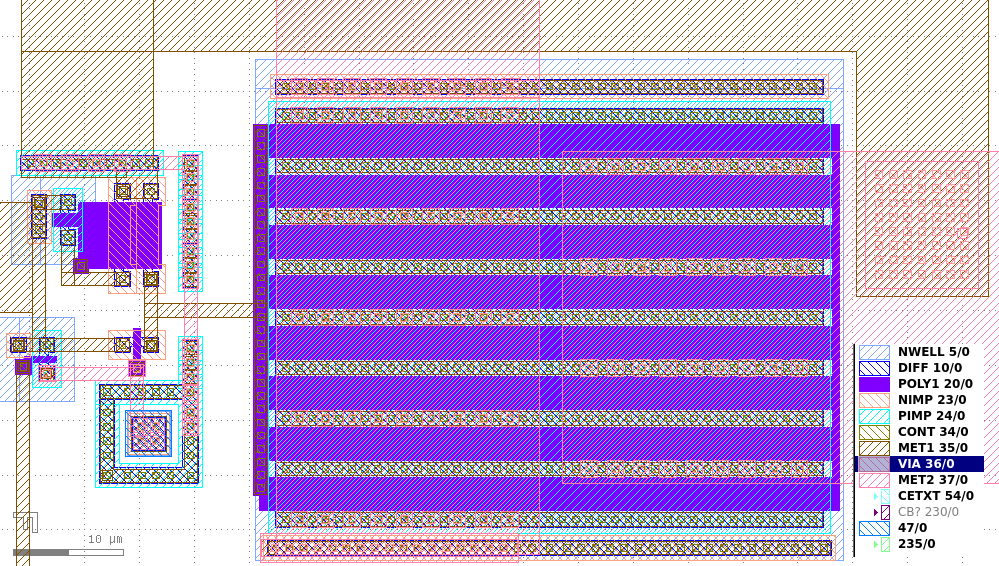
\includegraphics[width=\columnwidth]{figuras/gds/aps/todo.png}
    \caption{APS dosimeter layout.
    On the right is the output transistor, which belongs to the second follower stage.
    The rest can be seen in more detail in \figref{fig:layoutapszoom}.}
    \label{fig:layoutaps}
\end{figure}
\begin{figure}[p]
    \centering
    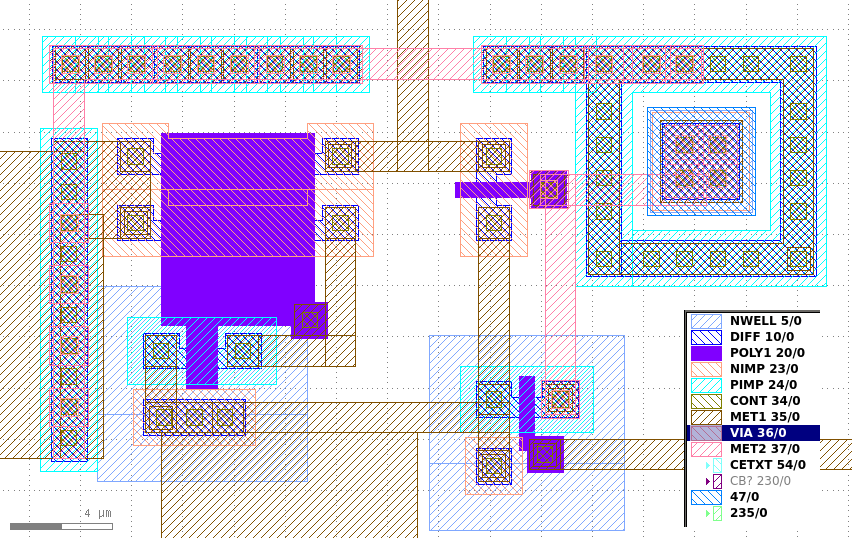
\includegraphics[width=\columnwidth]{figuras/gds/aps/zoom.png}
    \caption{Detail view of APS layout without the output transistor.
        To the right is the sensitive diode, with its N-well cathode at the center
        and anode (substrate) contacts all around it.
        To its left is the first follower stage transistor,
        and below it is the reset transistor.
        The transistors on the left provide the bias current for the first follower stage.
        The reset transistor is connected to a pad (not visible),
        through the protection circuit in\figref{fig:proteccion5v}.}
    \label{fig:layoutapszoom}
\end{figure}
\fig{proteccion5v}{figuras/aps/proteccion.pdf}
{Protection circuit for the reset input.
The diodes only turn on if the pad voltage exceeds
\SI{5}{\volt} or goes below \SI{0}{\volt}.
When a high-voltage pulse reaches the pad
(for example, due to electrostatic discharge),
the diodes prevent dangerous voltages from reaching the circuit.
This prevents any drain-body or source-body junctions from being forward-biased,
which might cause a latchup failure (section~\ref{latchup}).
It also protects MOS gate oxides from breaking down.}
\subsection{Measurement}
We wire-bonded two dies to a pair of TSSOP28 adapter boards.
These are small PCBs meant to adapt surface-mount components
to through-hole, for example to use them in a breadboard
(figures~\ref{fig:bondeados1}, \ref{fig:bondeados2} and~\ref{fig:pinout}).
\fig{bondeados1}{figuras/aps/bondeados.jpg}
{Bonded dies on SMD adapter board.
The boards are mounted on sockets which short-circuit all of the leads.
This protects the die from electrostatic discharge during transport and storage.
}
\figp{bondeados2}{figuras/aps/die.jpg}
{Close-up view of the die with the APS and FG dosimeters
(top of the center column)
, along with other circuits.}
\figp{pinout}{figuras/aps/pinout1.pdf}
{Layout of the complete die, including pinouts for the pads that were wire-bonded.}
\subsubsection{Self-discharge curves}
We first measured the sensor's output in the absence of light and radiation.
(figures~\ref{fig:oscuridad4} and~\ref{fig:oscuridad40}).
\fig{oscuridad4}{figuras/aps/oscuridad4.pdf}
{Self-discharge curve of the \SI{4}{\micro\meter} APS.
It is obtained by resetting the APS and measuring its output voltage in the dark.}
\fig{oscuridad40}{figuras/aps/oscuridad40.pdf}
{Self-discharge curve of the \SI{40}{\micro\meter} APS.
It is obtained by resetting the APS and measuring its output voltage in the dark.}
This shows us the discharge due to the diode's reverse leakage current.

Both variants of the APS have curves with similar shapes,
but with different time and voltage scales.
Their differences are mainly due to the disparity in diode area.
In addition, there are small differences (mismatch) between the MOS in the follower stages.
Each MOS has random variations due to imperfections in the processing steps
(mask, lithography, implantation, etc).
These variations tend to cancel out in large devices,
but are significant in minimum-area devices.
for example, the same absolute error in channel dimensions causes
a much bigger relative error in the channel current.
Since the first follower stage uses a minimum-area transistor,
it is particularly sensitive to mismatch and process variability.
% Descarga debería ser lineal
% https://books.google.com.ar/books?id=6Rg7AAAAQBAJ&lpg=PA289&ots=yO1HPv_N4E&dq=reverse%20biased%20diode%20%22discharge%20curve%22&hl=es&pg=PA290#v=onepage&q=reverse%20biased%20diode%20%22discharge%20curve%22&f=false

The self-discharge curve is the solution to a non-linear differential equation:
\begin{align*}
    \frac{\partial Q}{\partial V}\frac{dV}{dt} &= -I(V)
\end{align*}
The shape of the curve is due to the voltage dependence of both 
the leakage current $I(V)$ 
and the diode capacitance $\frac{\partial Q}{\partial V}(V)$.
Both vary with voltage due to the change in the width of the depletion region.
As the reverse voltage falls,
the depletion region becomes narrower.
The junction capacitance is inversely proportional to its width.
As its volume shrinks,
thermal generation of electron-hole pairs happens at a lower rate.
Both effects lead to a reduced leakage current,
as is visible at the end of the discharge curves.

Furthermore, there are second order terms which we did not
consider in our simplified analysis.
For example,
the reset transistor in the cut-off region is not a perfect open circuit,
but rather has a small leakage current.
This current tends to charge D1's cathode,
slowing down its discharge.
%
\subsection{LED illumination}
We measured discharge curves while illuminating the dies with a LED,
varying its supply current to achieve a wide range of light intensities
(figures~\ref{fig:led4} and~\ref{fig:led40}).
\fig{led4}{figuras/aps/descarga_led_4.pdf}
{Discharge curve under LED illumination for \SI{40}{\micro\meter} APS.
LED current increases from \SI{.1}{\milli\ampere} on the right to \SI{10}{\milli\ampere} on the left,
with 6 curves per decade.}
\fig{led40}{figuras/aps/descarga_led_40.pdf}
{Curva de descarga iluminando con un LED el APS de \SI{4}{\micro\meter} APS.
LED current increases from \SI{.1}{\milli\ampere} on the right to \SI{10}{\milli\ampere} on the left,
with 6 curves per decade.}

Esto permite observar la compresión en tiempo de la curva de descarga 
con el aumento de la radiación incidente.
No fue posible medir el efecto de otros tipos de radiación
(por ejemplo, $\beta$) por limitaciones de tiempo.
\subsubsection{Ruido medido}
Establecimos que una medición con este dosímetro consiste en promediar 10
muestras de tensión tomadas a una frecuencia de \SI{625}{\hertz} 
(período de muestreo \SI{1.6}{\milli\second}).
Al partir de esta definición,
estamos eligiendo no profundizar en
las características intrínsicas de ruido del sensor
(y su dependencia con la frecuencia, por ejemplo).
En cambio, nos enfocamos en el ruido que va a ver el usuario bajo ciertas
condiciones particulares de uso.

Con esta definición de qué es una medición, 
podemos definir de manera precisa el ruido como la desviación estándar
de ese promedio de 10 muestras.
Más precisamente, la tensión de salida a tasa de dosis constante
es la suma de una componente determinista $V_D$ y una aleatoria $\epsilon$
\begin{align*}
    V = V_D(\dot D, t) + \epsilon
\end{align*}. 
Al tomar la diferencia entre dos muestras consecutivas,
queda una pequeña componente sistemática 
(proporcional a $\Delta t\pderiv{V_D}{t}$) 
sumada a la diferencia entre dos variables aleatorias que suponemos
independientes.
Por lo tanto, 
la desviación estándar de la diferencia entre dos muestras consecutivas
es $\sqrt 2$ veces la desviación estándar presente en una muestra.

Para el análisis, medimos 6 disparos del APS
(cada disparo como las figuras~\ref{fig:led4} y~\ref{fig:led40}), 
totalizando 75000 muestras.
Luego diferenciamos estas mediciones y calculamos la desviación estándar.
Los resultados se ven en las figuras~\ref{fig:ruido4} y~\ref{fig:ruido40}.
% TODO: Las curvas medidas serían led4 y led40? Y pregunto:
% 1) Las miles de muestras corresponden a un disparo o a muchos disparos? Y
% cómo comparan los distintos disparos?
% 2) Cuál es el deltaT?

% TODO De dónde sale la equivalencia? ¿Es este sigma representativo de la
% dispersión en una repetición de disparos? Diría que está restringido a la
% freq de muestreo
\fig{ruido4}{figuras/aps/ruido4.pdf}{Ruido a la salida del APS de
    \SI{4x4}{\micro\meter}, calculado tomando diferencias entre muestras
    consecutivas y
escalando para que represente el ruido en un promedio de 10 valores.
La dosis equivalente se calculó con la sensibilidad proveniente
de las simulaciones SPICE y los cálculos de radiación.}
\fig{ruido40}{figuras/aps/ruido40.pdf}{Ruido a la salida del APS de
    \SI{40x40}{\micro\meter}, calculado tomando diferencias entre muestras
    consecutivas y
escalando para que represente el ruido en un promedio de 10 valores.
La dosis equivalente se calculó con la sensibilidad proveniente
de las simulaciones SPICE y los cálculos de radiación.}
También es posible tomar la desviación estándar para cada disparo,
como se ve en las figuras~\figref{fig:ruido_disparo_4} y~\figref{fig:ruido_disparo_40}.
Así se verifica que todos los disparos tienen una estadística similar.
\fig{ruido_disparo_4}{figuras/aps/std_disparo_aps4.pdf}
{Ruido a la salida del APS de \SI{40x40}{\micro\meter},
calculado usando muestras de disparos individuales.
Los resultados se agrupan muy cerca del valor de la \figref{fig:ruido40}.}
\fig{ruido_disparo_40}{figuras/aps/std_disparo_aps40.pdf}
{Ruido a la salida del APS de \SI{4x4}{\micro\meter},
calculado usando muestras de disparos individuales.
Los resultados se agrupan muy cerca del valor de la \figref{fig:ruido4}.}
Podemos convertir estos valores de ruido en dosis usando la sensibilidad
calculada en~\ref{section:diseno_aps}.
Así llegamos a una resolución de \SI{2.0}{\milli\gray} y \SI{2.3}{\milli\gray}
para el APS de \SI{4x4}{\micro\meter} y \SI{40x40}{\micro\meter},
    respectivamente.
Sin embargo, esto está restringido a 
las condiciones de muestreo de las que partimos,
y es posible hacer un análisis más general de 
la magnitud del ruido en función de la frecuencia.
Esto permitiría elegir otra cantidad de promediado o frecuencia de muestreo 
que logre mayor resolución.

Este análisis del ruido tampoco contempla todas los formas posibles
de usar el APS.
Su validez principal es al realizar una medición Correlated Double Sampling,
restando la tensión final a la tensión luego del reset.
Sin embargo,
también existe la posibilidad de medir durante intervalos largos,
sumando la dosis medida en cada ciclo de reset y descarga.
En este caso, se suma el error en cada disparo para llegar a un valor de ruido
proporcional a la raíz de la cantidad de disparos.

A fin de evaluar la repetitividad de la lectura, comparamos la tensión de salida de los APS un tiempo fijo después de su reseteo, para varios disparos.
El resultado (figuras~\ref{fig:comparacion_salida_disparos_aps4} y~\ref{fig:comparacion_salida_disparos_aps40}) es que hay una diferencia entre disparos de \SI{20}{\milli\volt} en el APS de \SI{4x4}{\micro\meter} y de \SI{12}{\milli\volt} en el de \SI{40x40}{\micro\meter}.
\fig{comparacion_salida_disparos_aps4}
{figuras/aps/tension_salida_comparando_disparos_aps4.pdf}
{Tensión de salida para varios disparos, un tiempo fijo luego de resetear el APS de \SI{4x4}{\micro\meter}.}
\fig{comparacion_salida_disparos_aps40}
{figuras/aps/tension_salida_comparando_disparos_aps40.pdf}
{Tensión de salida para varios disparos, un tiempo fijo luego de resetear el APS de \SI{40x40}{\micro\meter}.}
Si bien es una muestra reducida, la repetitividad de la lectura entre disparos es buena.
En particular, es comparable con el ruido de medición caracterizado en las figuras~\ref{fig:ruido_disparo_4} y~\ref{fig:ruido_disparo_40}.
Las lecturas están acotadas en un intervalo de \SI{20}{\milli\volt} para el dispositivo de \SI{4x4}{\micro\meter} y es aproximadamente la mitad en el dispositivo de \SI{40x40}{\micro\meter}; valores comparables con las desviaciones estándar obtenidas para la dispersión de las lecturas intra-disparos.
%
\subsection{Resúmen de características}
El dosímetros APS de \SI{4x4}{\micro\meter} que diseñamos, 
fabricamos y construímos presenta las
siguientes características:
\begin{itemize}
    \item Sensibilidad: \SI{7.1}{\volt\per\gray}
    \item Resolución: \SI{2.0}{\milli\gray}
    \item Rango (por disparo): \SI{0.4}{\gray}
\end{itemize}
%
\subsection{Conclusiones}
Presentamos el concepto básico del dosímetro APS,
con sus peculiaridades de uso y el tipo de mediciones que permite realizar.
Cubrimos su teoría de funcionamiento,
y de ahí explicamos el proceso de diseñar el circuito
para su fabricación.

En los resultados verificamos que el sensor
sigue el comportamiento básico que esperamos,
tanto en ausencia de radiación 
como para distintas intensidades de luz visible.
Asimismo, conseguimos una estimación inicial de la resolución del sensor
en base al ruido medido a la salida.
Así dimos los primeros pasos para implementar un dosímetro APS
en un proceso de fabricación CMOS estándar.
